\documentclass[a4paper, 12pt]{report}
\usepackage[margin=1in]{geometry}
\usepackage{amsfonts, amssymb,amsmath}
\usepackage{setspace}
\usepackage{graphicx}
\usepackage{float}
\usepackage{hyperref}


\title{COMPARISON OF STARLINK ISP WITH MIKROTIK TECHNOLOGY}
\author{BY \\
		AKPALA SOMTOCHUKWU EKOJOKA\\
		AKHIHIERO VICTOR ILEVBARE}
\date{DEPARTMENT OF ELECTRICAL/ELECTRONICS ENGINEERING\\
FACULTY OF ENGINEERING\\
UNIVERSITY OF BENIN\\
BENIN CITY}
\begin{document}
\maketitle
\chapter*{ABSTRACT}
Considering the unique context of Nigeria, this paper explores the operational intricacies of the Low Earth Orbit (LEO) satellite system Starlink and does a comparison analysis with classic Geostationary Earth Orbit (GEO) satellite systems. This study used a qualitative technique to examine many performance characteristics, such as Jitter, Packet Loss, Throughput, Routing Strategy, Latency, Generic Data Transfer, and Environmental Influential Factors.\\ \\
Our goal is to provide significant insights into the real-world uses and consequences of Starlink's technology in Nigeria through this research. It is anticipated that the results would provide insight into the performance dynamics of satellite systems to academics, stakeholders, enabling them to make well-informed decisions in the constantly changing telecommunications industry.

\chapter*{DEDICATION}
\begin{doublespacing}
\chapter{INTRODUCTION}
\section{Context Of Study}
History has it that in August 1962, J.C.R. Licklider of MIT wrote a series of memoranda outlining his ``Galactic Network" concept, which was the first documented account of the social connections that networking could facilitate. \cite{leinerbrief}. In the course of the Cold War, the internet was used as a government project to establish communication in the military that could not be damaged by a nuclear bomb \cite{abbate2000inventing}. After the war, modern day internet was born. On April 30, 1995, the American government halted operations of the old NSFNET backbone and handed over the infrastructure to private companies \cite{abbate2000inventing}.\\
	According to \cite{mack2020history} the mode of connection to this early internet was through modems connected over telephone line charging in per use basis at a speed of 33.6kbps and 56 kbps. This means that it would take 1 day, 18 hours and 36 minutes to download a 1 gigabyte file. As the need for faster internet became more glaring, broadband became available to the public with better speed and constant connection unlike modems which require dial-up before connection\\.
	\cite{moeyaert2011network} explains that there are roughly five types of broadband connection technologies currently in use. Among them are Digital Subscriber Line (DSL), cable modem, fibre, wireless, satellite, and broadband over power lines.\\
	Satellite broadband, which is our focus, was first considered for internet usage in 1986 by Via-Sat, a company started by Mark Dankberg, Steve Hart, and Mark Miller (\href{https://news.viasat.com/blog/scn/satellite-communications-a-brief-history-from-sputnik-to-viasat-3}{``Satellite Communications: A Brief History From Sputnik to ViaSat-3''}). With the technology developing rapidly, companies ventured into satellite broadband using Geographical Earth Orbit (GEO) satellites, but it came with some disadvantages, yielding to the exploration of satellite broadband using Low Earth Orbit (LEO) satellites.\\
	SpaceX Starlink, a satellite internet service provider licenced for operation in May 2022 in Nigeria (NCC 2023), has raised questions concerning her reliability to deliver better internet performance for Nigerians, where the need for fast internet is rampant as technology develops rapidly.
	The regular internet service providers in Nigeria, employs GEO technology where ground stations communicates with the satellite orbiting 35,786km from the earth's surface. This approach of internet connection is said to be characterized by slow speed and it has high latency and longer routing strategy.
	To offer a solution, a more recent approach to internet connectivity has been developed, being employed by SpaceX Starlink - the LEO (Low Earth Orbit) Satellite.
	Starlink satellites are LEO, meaning they are launched to an orbit about 550km away from the earth, which is a distance much closer to the Earth compared to GEO satellites. With this, Starlink is excepted to have better performance in terms of Latency, Routing Strategy and Throughput as the distance is shorter and direct communication with the satellite dish (Dishy) is made possible.\\
	For Starlink broadband to function, it requires the communication between a Starlink internet antenna or Starlink dish antenna called Dishy Mcflatface (Dishy for short) which is placed in an obstruction-free location and a Starlink satellite orbiting at a speed of 27000km/hr in the LEO.
	The Dishy is made of sturdy, temperature- and weather-resistant material that can tolerate harsh weather. It consists of various layers but most importantly, 1280 antennas which are arranged in a hexagonal honeycomb pattern. Communication with the fast moving satellite is made possible by including phased array technology which helps steer the beams from the antennas without physically moving it. Various versions of Dishy have been launched, with a visible difference in flatness and size thereby making Starlink suitable for mobility\\
	The first lunched Starlink requires the user to be about 50km from ground stations also known as gateways. This  is necessary because Dishy needs to communicate with the ground station with its required data which is then related to the Starlink satellite before the later transmits to the Dishy; It is termed bentpipe architecture. Version 2 Satellites launched in April 2023 are equipped with LASER communication to enable the satellite communicate between themselves in orbit, thereby limiting the need for ground stations.
	
\begin{figure}[H]
\centering
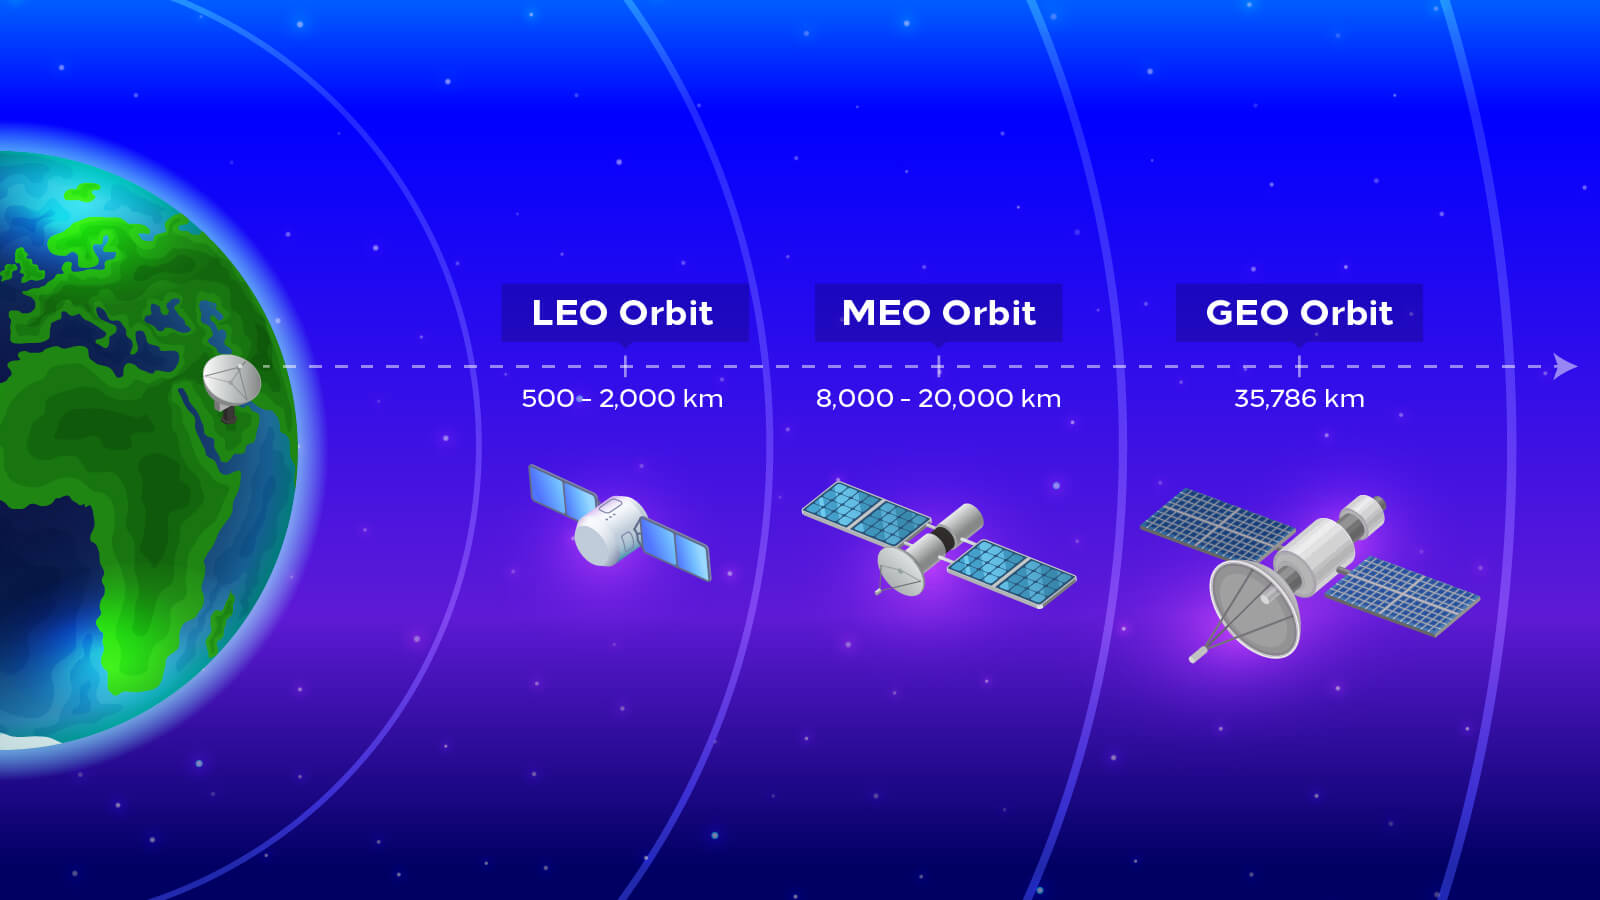
\includegraphics[width=0.9\textwidth]{space orbits}
\caption{Types of Satellite Constellations}
\end{figure}

\section{Motivation for Study}
The dynamic nature of satellite technology and its potential to alleviate Nigeria's connection issues are the driving forces behind this research.\\
The need to overcome connectivity gaps in Nigeria's underprivileged and  isolated areas is what spurred this research. Access to dependable internet connectivity is a critical issue in many parts of the nation, especially in isolated and economically disadvantaged communities.
A major obstacle for the typical Nigerian is Starlink's relatively high cost, which ranges from ₦290,000 to ₦350,000. Given the few empirical research done to verify the product's claimed capabilities and performance, this cost barrier is particularly noteworthy. In Nigeria, a nation with a diverse population of economic origins, affordability plays a crucial role in the broad adoption of technology solutions. It is unclear whether the product's true performance and advantages outweigh its cost due to the lack of a thorough empirical investigation. Potential customers would be reluctant to purchase Starlink if there is no empirical support for the high cost, as the product's perceived value may not match what it costs.\\
This study seeks to bridge this gap by conducting an in-depth examination of Starlink's performance, taking into account factors such as latency, throughput, and browsing performance. This helps to clarify the practicality of Starlink and provides a baseline for further research in the area.\\
Quite a number of people have tried measuring Starlink's performance in high internet speed demanding platforms such as gaming and streaming. It is important to state that their review from such tests cannot be free from major errors as the performance is not in it's totality dependent on the broadband, as there could be external influences too. Hence this research to empirically do testing that follows proper scientific procedures.

\section{Aim of study}
The goal of this research is to undergo a thorough analysis of Starlink's performance indicators, encompassing browsing speed, latency, reliability, and coverage, in the context of Nigeria's unique environmental and infrastructural constraints. This assessment is expected to yield significant information regarding Starlink's flexibility and reliability in tackling the various connectivity obstacles encountered around the nation. This study additionally contributes significant insight that not only indicates the particular performance of Starlink in Nigeria but also lays the groundwork for strategic planning and well-informed decision-making within the rapidly changing satellite communication market in that nation.

\section{Scope}
The geographic scope of this exploration is intricately tied to Nigeria, offering a detailed examination of how Starlink operates in this environment. This research is centered on examining how Starlink operates and evaluating its performance. \\
The analysis delves into key technical performance metrics such as speed, latency, reliability, and coverage, considering the environmental and infrastructural conditions unique to Nigeria.\\
Unlike an exhaustive exploration of the underlying technological complexities, this study refrains from delving into the minute details already covered in dedicated articles. Instead, it emphasizes understanding the practical applications and implications of Starlink's technology.\\
Lastly, this research is singularly focused on one specific Starlink dish model – the rectangular (square) Starlink Dishy. Findings and conclusions drawn will be confined to this particular model, ensuring a targeted and in-depth investigation.\\
\section{Methodology}
This study uses qualitative research methodologies to assess the practical performance of Starlink, focusing on a comprehensive and detailed analysis within the Nigerian setting. The technique provides specific insights through the measurement and analysis of various performance metrics, such as:
\begin{enumerate}
\item Latency
\item Throughput
\item Packet Loss
\item Routing Strategy
\item Jitter
\item Generic Data Transfer
\item Environmental Influential Factors
\end{enumerate}

\end{doublespacing}
\bibliographystyle{apalike}
\bibliography{Reference/bib_file}
\end{document}